\section{GPU}

\frame{\frametitle{Index}\tableofcontents[currentsection]}

%
% IMPLEMENTATION
%
\frame{\frametitle{GPU}

	\begin{block}{Implementation}
		\begin{itemize}
			\item \textit{Struct-of-Arrays}

			\item \texttt{compute\_flux} and \texttt{update} directly converted to CUDA Kernels
			\begin{itemize}
				\item[-] Each iteration translates to one CUDA Thread
			\end{itemize}

			\item One additional \texttt{reduction} kernel (later removed)

			\item Data transfers only happen before the main loop
			\begin{itemize}
				\item[] (exception: animation output, which is disabled)
			\end{itemize}
		\end{itemize}
	\end{block}
	\pause


	\begin{block}{Load Balance}
		\begin{itemize}
			\item workload of both kernels is homogeneous
			\begin{itemize}
				\item[] (exception: \update, if number of edges per cell differs)
			\end{itemize}
		\end{itemize}
	\end{block}
}

\frame{\frametitle{GPU}
	\begin{block}{Optimizations}
		Several versions tested, each with new tweaks
		\begin{itemize}
			\item Temporary variables and avoidance of memory accesses
			\item Divergence avoidance
			\item A division in \update was replaced by precomputed values
			\begin{itemize}
				\item[] More memory required, but divisions are not GPU-friendly
			\end{itemize}
		\end{itemize}
	\end{block}
	\pause

	\begin{block}{Global kernel speedups}
		\begin{table}
			\begin{tabular}{r|cc|c}
							&	Initial	&	Optimal	&	Speedup	\\ \hline
			\computeflux	&	0.72	&	0.7		&	\textbf{1.03}	\\
			\update			&	3.60	&	1.96	&	\textbf{1.84}	\\ \hline
			\end{tabular}
			\caption{Comparison of first and last kernel implementations. Times are in ms.}
		\end{table}
	\end{block}
}

% \begin{frame}
% 	\frametitle{Results}
% 	\begin{figure}
% 		\centering
% 		\includegraphics[width=0.8\textwidth]{graph_comparison_.eps}
% 	\end{figure}
% \end{frame}

\frame{\frametitle{Results}
	\begin{figure}
		\centering
		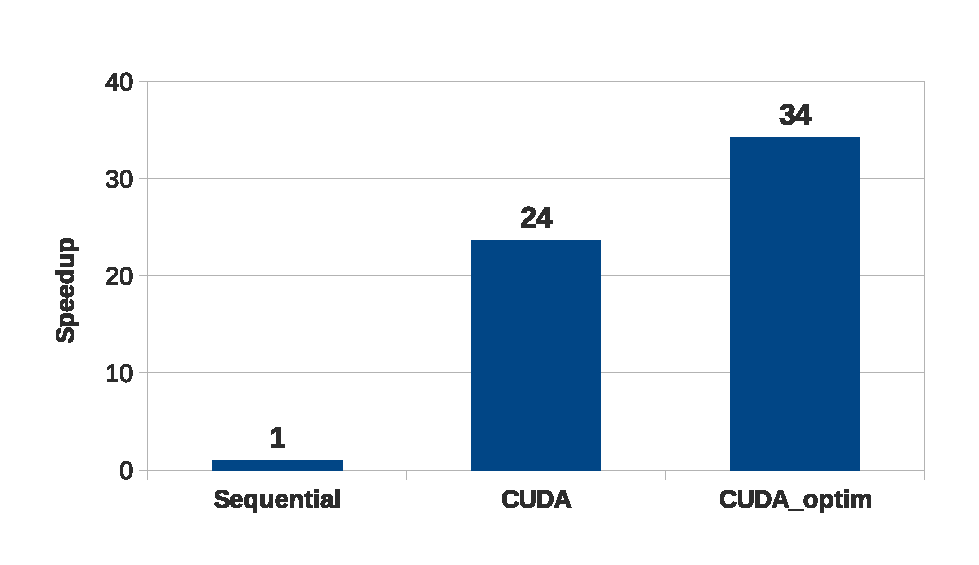
\includegraphics[width=0.8\textwidth]{graph_comparison_cuda.eps}
	\end{figure}
}

\frame{\frametitle{GPU}

	\begin{block}{Limitations}
		\begin{itemize}\itemsep=20pt
			\item Memory accesses are the main issue
			\begin{itemize}
				\item[-] \computeflux will not access cells in order
				\item[-] Same problem for \update when accessing edges
			\end{itemize}
			\pause

			\item Locality issues
			\begin{itemize}
				\item[-] largely due to unorganized \texttt{gmsh} output
			\end{itemize}

		\end{itemize}
	\end{block}
}

\begin{frame}[fragile]
	\frametitle{\texttt{gmsh} locality issues}

	Pollution values initialized with:
	\begin{center}
		\begin{verbatim}
			pollution[cell_index] = cell_index
		\end{verbatim}
	\end{center}
	\pause

	Closer colors indicate closer cells in memory:

	\begin{figure}
		\centering
		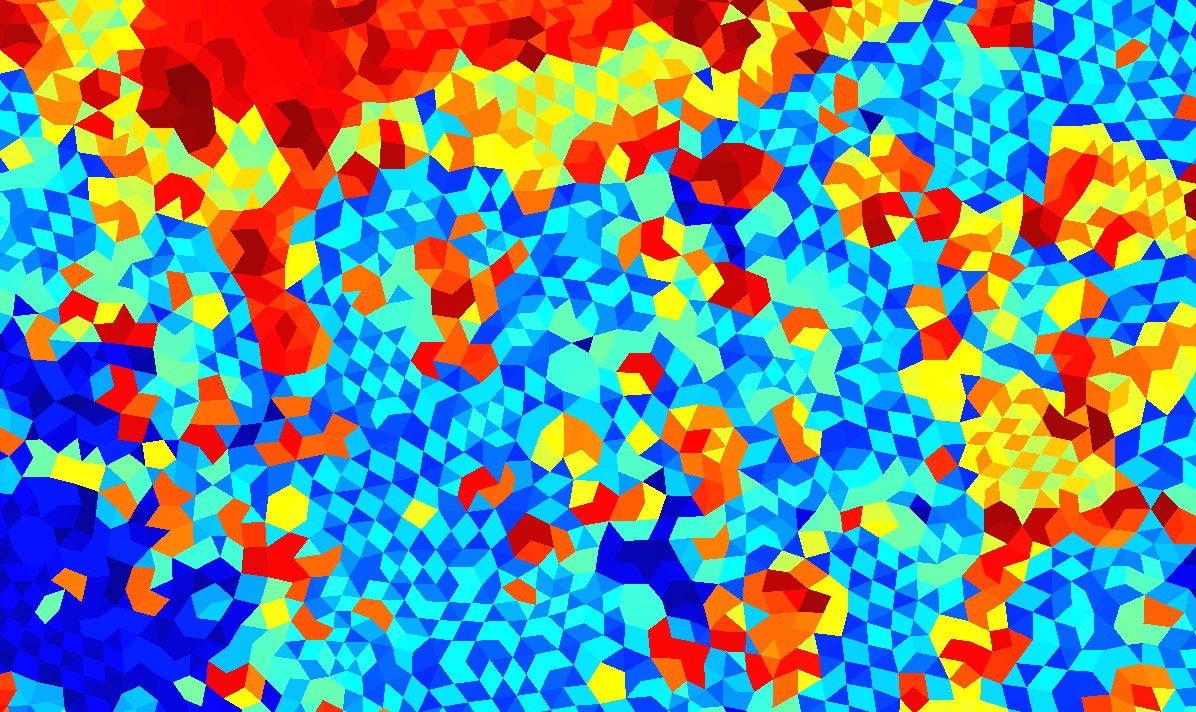
\includegraphics[width=0.8\textwidth]{locality_big}
	\end{figure}
\end{frame}

